\section[C'est quoi, Internet ?]{Mais au fait, c'est quoi, Internet ?}

\subsection{Le concept général}

\begin{frame}{D'où vient cette idée bizarre ?}
  \begin{figure}
    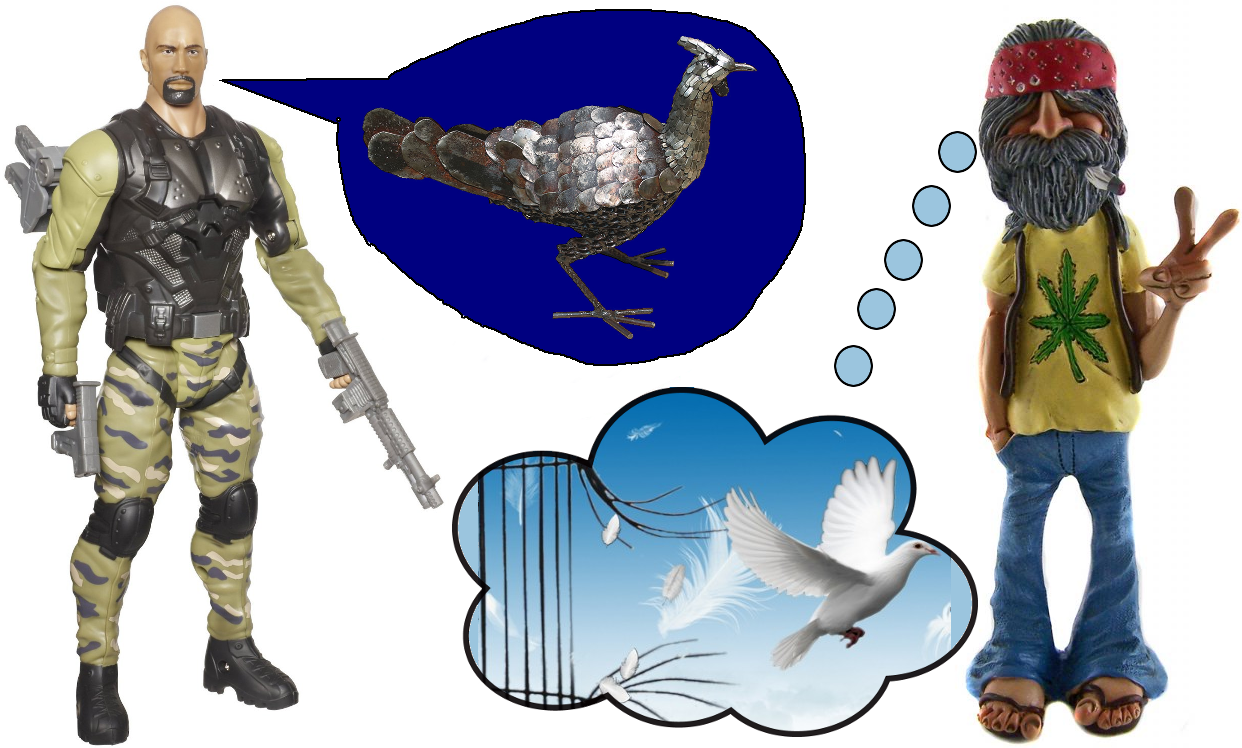
\includegraphics[width=0.9\textwidth]{concepts/usarmy.png}
  \end{figure}
\end{frame}

\begin{frame}{Indestructible ? Donc pas comme ça !}
  \begin{textblock*}{0.25\textwidth}(0.9\textwidth,0.7\textheight)
    
\includegraphics[width=\textwidth]{concepts/trainwestern.png}
  \end{textblock*}
  \centering
  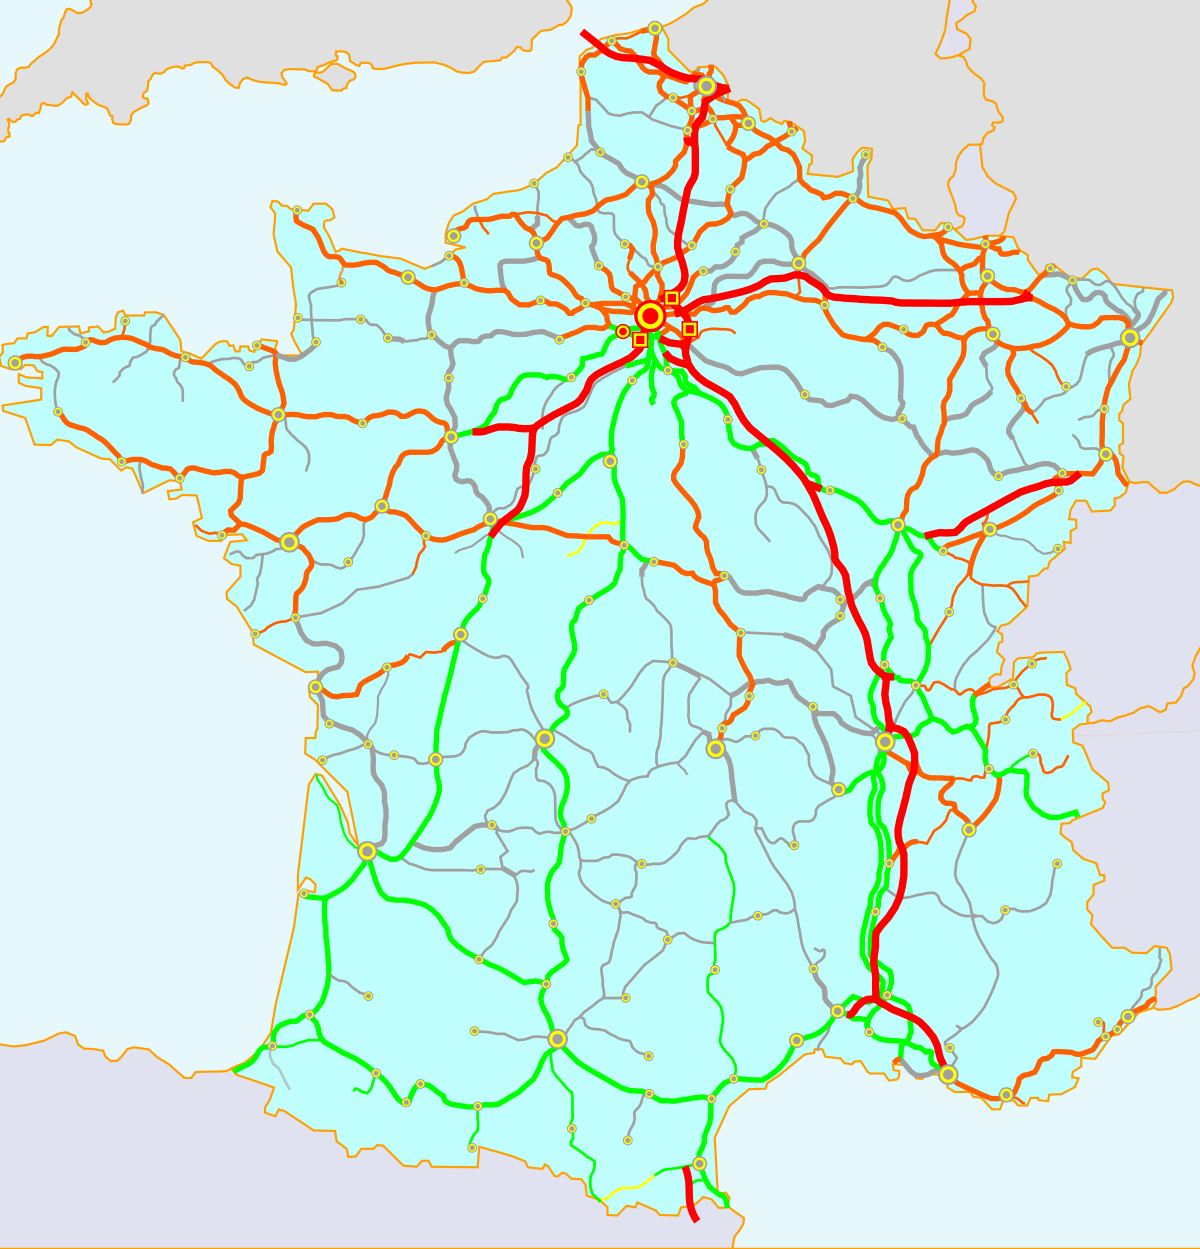
\includegraphics[height=0.8\textheight]{concepts/france.png}
\end{frame}

\begin{frame}{Mais si on en met plusieurs ?}
  \begin{textblock*}{0.25\textwidth}(0.9\textwidth,0.7\textheight)
    
\includegraphics[width=\textwidth]{concepts/trainwestern.png}
  \end{textblock*}
  \centering
  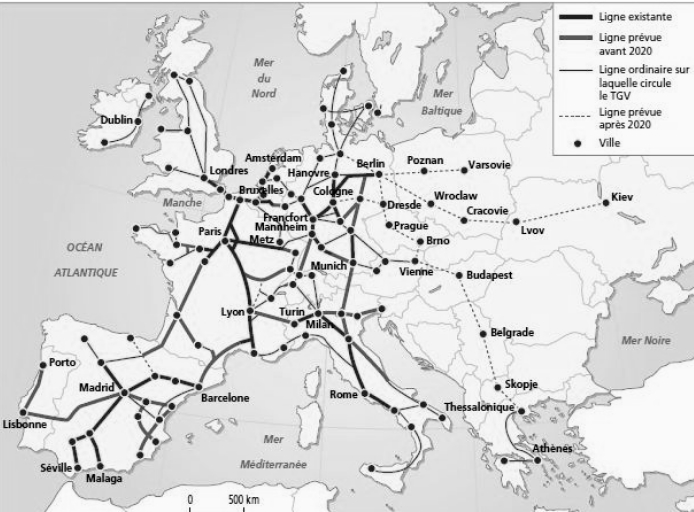
\includegraphics[height=0.8\textheight]{concepts/europe.jpg}
\end{frame}

\subsection{Quelques règles de fonctionnement}

\begin{frame}{Allez, plus en détails :}
  \begin{columns}
  \begin{column}{0.7\textwidth}
    \hspace{5em}Mail\hspace{4em}Web\hspace{3em}P2P
    \vspace{-1em}
    \begin{figure}
      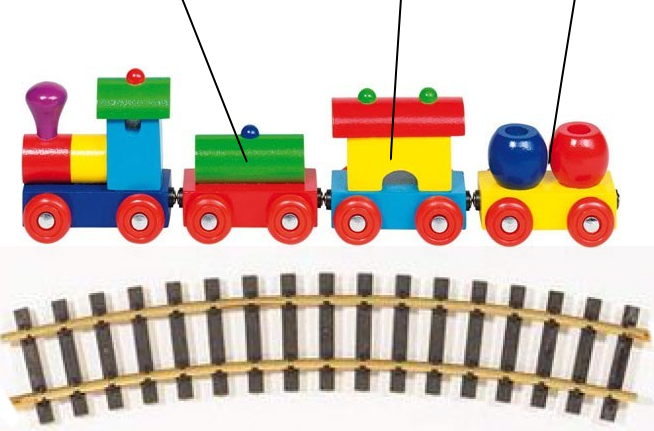
\includegraphics[width=0.9\textwidth]{concepts/protocoles.png}
    \end{figure}
  \end{column}
  \begin{column}{0.4\textwidth}
    \begin{itemize}
      \vspace{2em}
      \item Protocoles et données
      \item Couche IP
      \vspace{2em}
      \item Réseau physique
    \end{itemize}
  \end{column}
  \end{columns}
\end{frame}

\begin{frame}{\hfill(en vrai, il n'y a pas qu'un seul train)}
  \begin{figure}
    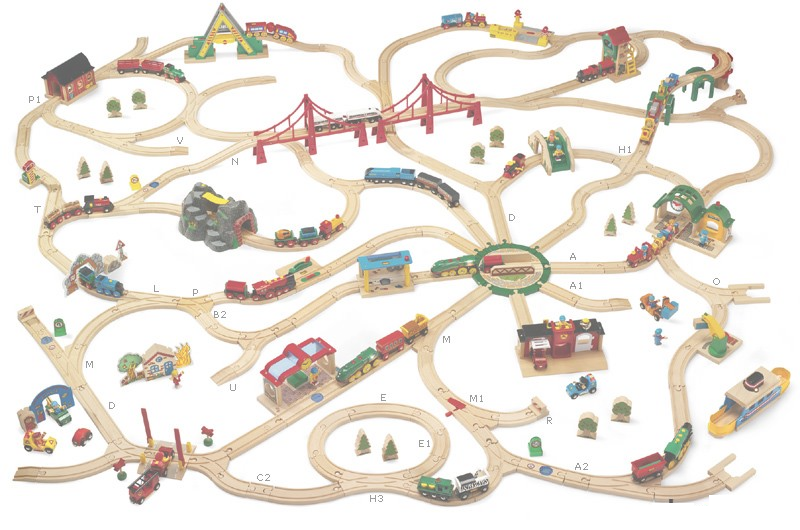
\includegraphics[width=\textwidth]{concepts/rails.png}
  \end{figure}
  \begin{textblock*}{8em}(0.8\textwidth,0.2\textheight)
    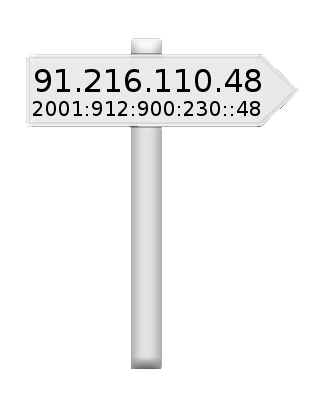
\includegraphics[width=\textwidth]{concepts/ipdirection.png}
  \end{textblock*}
  \begin{textblock*}{12em}(0.3\textwidth,0.3\textheight)
    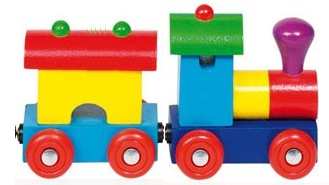
\includegraphics[width=\textwidth]{concepts/paquet.png}
  \end{textblock*}
  \begin{textblock*}{12em}(0.0\textwidth,0.5\textheight)
    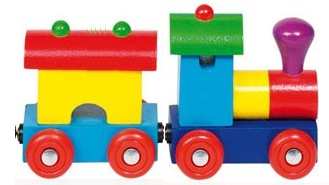
\includegraphics[width=\textwidth]{concepts/paquet.png}
  \end{textblock*}
  \begin{textblock*}{12em}(0.5\textwidth,0.5\textheight)
    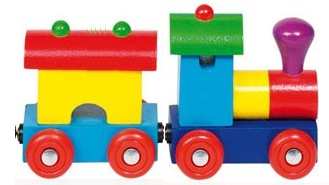
\includegraphics[width=\textwidth]{concepts/paquet.png}
  \end{textblock*}
  \begin{textblock*}{12em}(0.2\textwidth,0.7\textheight)
    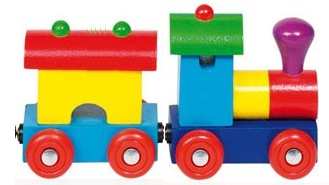
\includegraphics[width=\textwidth]{concepts/paquet.png}
  \end{textblock*}
\end{frame}

\begin{frame}{Une communication par paquets}
  \begin{figure}
    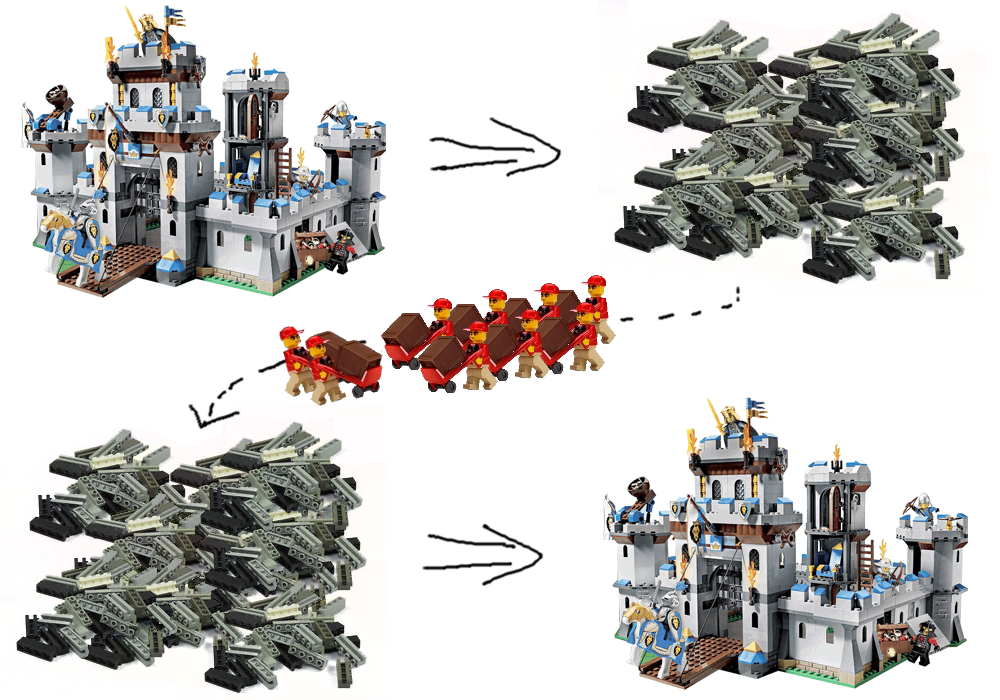
\includegraphics[width=0.9\textwidth]{concepts/lego-paquets.png}
  \end{figure}
\end{frame}

\subsection{Ça donne quoi en pratique ?}

\begin{frame}{Plusieurs routes disponibles…}
  \begin{figure}
    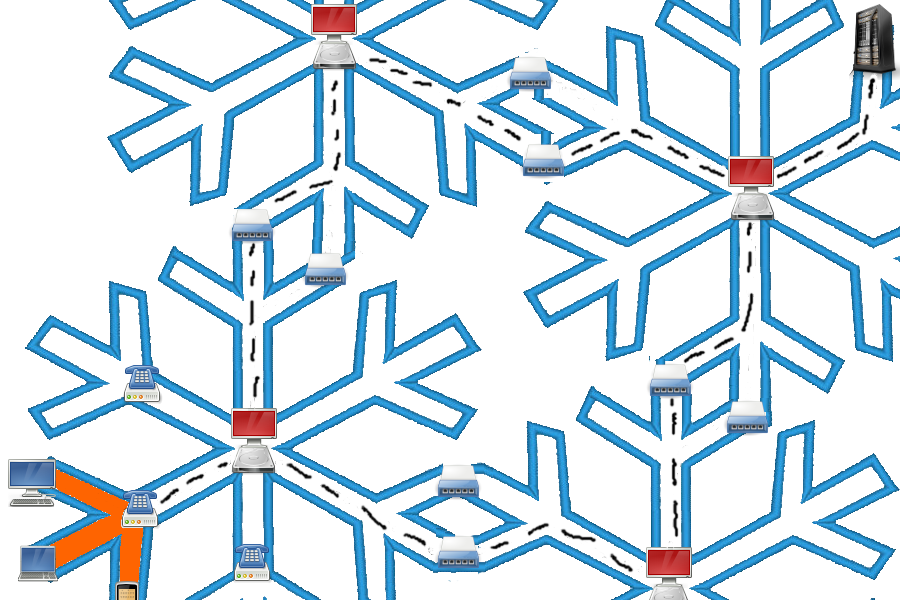
\includegraphics[width=0.9\textwidth]{concepts/flocon-trajet.png}
  \end{figure}
\end{frame}

\begin{frame}{\textit{\textbf{Inter}connection of \textbf{Net}works}}
  \begin{figure}
    \vspace{-0.9em}
    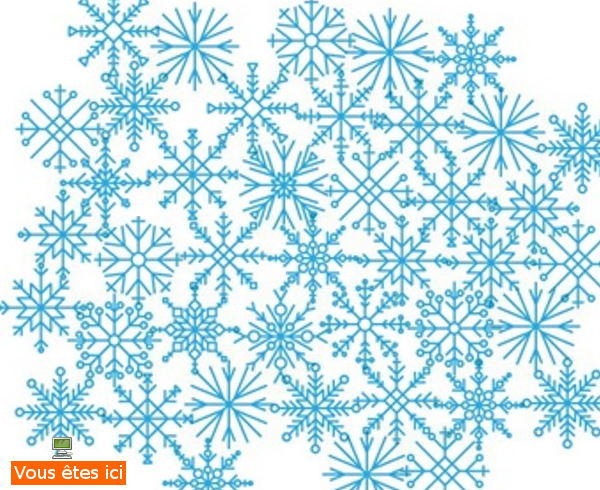
\includegraphics[width=0.9\textwidth]{concepts/flocon-total.png}
  \end{figure}
\end{frame}

\begin{frame}{Si on dessine autrement…}
  \begin{textblock*}{0.28\textwidth}(0.92\textwidth,0.5em)
    
\includegraphics[width=\textwidth]{concepts/rfc1149.png}
  \end{textblock*}
  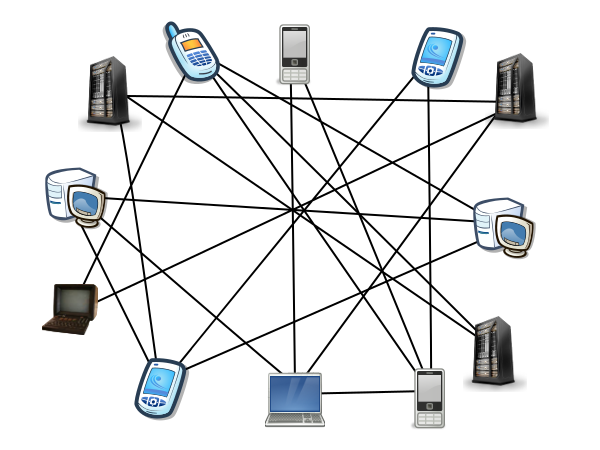
\includegraphics[width=0.9\textwidth]{concepts/reseau-bazar.png}
\end{frame}
